\documentclass[dvipdfmx,11pt]{beamer}
\graphicspath{{_images/}{../_images/}}
\usepackage{lipsum}
\usetheme{verona}
\usepackage{bxdpx-beamer}
\usepackage{pxjahyper}
\usepackage{minijs}
\usepackage{mathpazo}
\usepackage{amsmath,amssymb}
\usepackage{graphicx}
\usepackage{array}
\usepackage{tikz}
\setbeamertemplate{navigation symbols}{}

\title{Shocking Racial Attitudes: \\ Black G.I.s in Europe}
\subtitle{Schindler and Westcott (2020, REStud)}
\author{Reviewed by Reio TANJI}
\date{Oct 27th 2020 \\ Ohtake-Sasaki Seminar}
\institute{Osaka University, Graduate School of Economics}

\begin{document}
\begin{frame}\frametitle{}
\titlepage
\end{frame}


\begin{frame}\frametitle{Abstract}
  \begin{itemize}
      \item Research Question: Can attitudes toward minorities be changed?
      \item Method: Regression using empirical dataset of US army units in the UK.
      \item Sum of the results: Presence of African American soldiers in the UK during World War II reduced anti-minority prejudice.
      \begin{itemize}
        \item  as a result of the positive interactions.
      \end{itemize}
  \end{itemize}
\end{frame}

\section{Introduction}
\begin{frame}\frametitle{Introduction}
  \begin{itemize}
    \item Prejudicial attitudes toward minority groups are widespread, and persists over the very long run (Voigtl\"{a}nder and Voth, 2012; Acharya et al., 2016)
    \item Less is known about:
    \begin{itemize}
      \item what it takes to change such attitudes.
      \item whether any such changes in attitudes might themselves persist.
    \end{itemize}
    \item This is important to understand the consequences
    \begin{itemize}
      \item social conflict
      \item hate crime
      \item labour and goods market discrimination.
    \end{itemize}
  \end{itemize}
\end{frame}

\begin{frame}\frametitle{G.I.s in the UK}
  \begin{itemize}
    \item During World War II, the UK played host to over one and a half million US troops, including 150,000 African Americans.
    \begin{itemize}
      \item Serving with non-combat support duties such as transport and supply.
      \item Many Britons saw and interacted with non-whites for the very first time.
      \begin{itemize}
        \item Frequently found in pubs, dance halls, and Restaurants (Millgate, 2010)
      \end{itemize}
    \end{itemize}
    \item A newly constructed dataset of US military bases in the UK and present-day measures of anti-minority preferences show:
    \begin{itemize}
      \item Individuals in areas of the UK where black troops were posted are more tolerant towards minorities 60 years ofter the last troops left.
      \begin{enumerate}
        \item Fewer members of the British National Party (BNP).
        \item Residents are less likely to vote Conservative in local elections.
        \item Less implicit anti-black bias measured by Implicit Association Test (IAT) scores.
      \end{enumerate}
    \end{itemize}
  \end{itemize}
\end{frame}

\begin{frame}\frametitle{Contribution}
  \begin{itemize}
    \item \textbf{Contact Hypothesis (Allport, 1954)}: Contact with minorities can reduce prejudice.
    \begin{itemize}
      \item Boisjoly et al.(2006); Carell et al.(2019); Burns et ak.(2016): assigning non-white roommates to white students at higher education

      $\Rightarrow$ meaningful effect on broader cross-section of the population.
    \end{itemize}
    \item \textbf{Cultural norms}: Preferences are endogenous to social and family environments.
    \begin{itemize}
      \item Path of preference formation: vertical and horizontal transmission of values (Bisin and Verdier, 2001).
      \item Very long-run persistence in preferences (Voigtl\"{a}nder and Voth, 2012; Archarya, 2016)

      This paper: contact as an important potential source for persistent changes in attitudes/cultural norms (Fouka, 2020).
    \end{itemize}
  \end{itemize}
\end{frame}

\begin{frame}\frametitle{}
  \begin{itemize}
    \item \textbf{Historical determinants of support for far-right parties}
    \begin{itemize}
      \item Political alienation increase support for radical far-right parties.(Vlanchos, 2017)
      \item The effect is persistent (Ochsner and Roesel, 2020; Cantoni et al., 2019)

      This paper: a high level intergenerational correlation in attitudes towards migration and support for far-right parties (Avdeenko and Siedler, 2017).
    \end{itemize}
    \item \textbf{Effect of a historical event on implicit attitudes as measured by a computerized IAT}
    \begin{itemize}
      \item Implicit attitudes against minority groups are increasingly used in the economics literature to measure bias, and predictive of behavior (Greenwald and Banaji, 1995; Lowes et al., 2015).
      \item Historic events can shape implicit attitudes (Lowes and Montero, 2016; Lowes et al., 2017).
    \end{itemize}
  \end{itemize}
\end{frame}

\section{Historical Overview}
\frame{\sectionpage}
\begin{frame}\frametitle{US army in the UK}
  \begin{tabular}{ll}
    \begin{minipage}{.45\textwidth}
      \begin{figure}[ht]
        \centering
        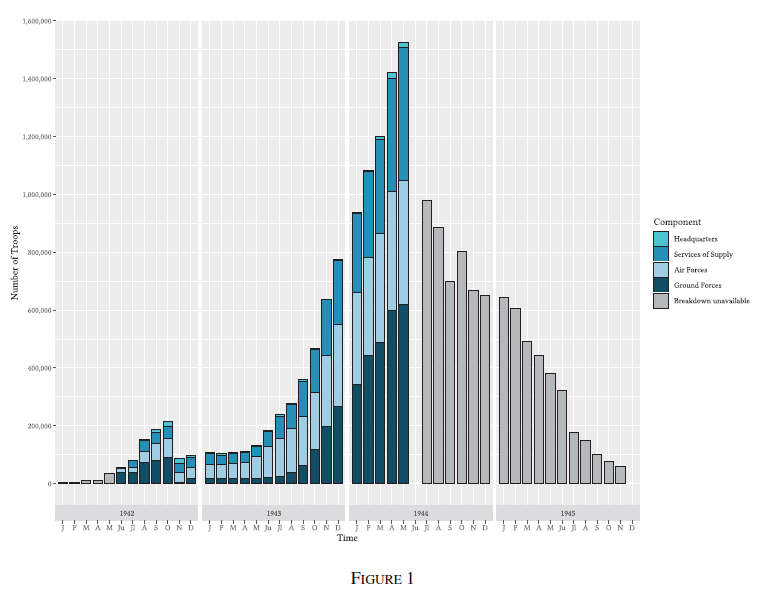
\includegraphics[scale = .45]{os1027tanji/f1}
      \end{figure}
    \end{minipage} &
    \begin{minipage}{.5\textwidth}
      \begin{itemize}
        \scriptsize
        \item December 1941: The US entered WWII
        \item May 1942: preparation for a land offensive.
        \item May 1943: Plans for a 1944 offensive were settled.
        \item June 1944: Most American troops left in the Course of "Operation Overload," but troop numbers did not decrease until the end of the war.
        \item November 1945: almost all American units had left the UK.
      \end{itemize}
    \end{minipage}
  \end{tabular}
\end{frame}

\begin{frame}\frametitle{Black G.I.s}
  \begin{itemize}
    \item Over 900,000 African Americans served in the US military during World War II.
    \begin{itemize}
      \item With few exceptions, black troops were limited to non-combat “labour” or “service” roles.
      \item around 10\% of G.I.s who served in the UK were African American.
    \end{itemize}
    \item Around 50\% of African Americans had no high school education
    \begin{itemize}
      \item a relatively moderate positive selection with respect to the young black male population as a whole
    \end{itemize}
    \item Black soldiers served in racially segregated units, normally under command of white officers.
    \begin{itemize}
      \item Minimum interaction between black and white soldiers with accommodation, dining and training facilities all segregated.
    \end{itemize}
    \item Evidence suggests that frequent contact between soldiers and local populations took place.
  \end{itemize}
\end{frame}

\section{Evidence on Contact}
\frame{\sectionpage}
\begin{frame}\frametitle{Interaction between the Black G.I.s and the Locals}
  \begin{itemize}
    \item In most areas of the UK where black G.I.s were stationed, locals would have been seeing and interacting with black people for the first time.
    \item The evidence suggests that the British responded positively to black G.I.s.
    \begin{itemize}
      \item 'the general consensus of opinion seems to be that the only American soldiers with decent manners are the Negroes' (Orwell, 1943)
    \end{itemize}
    \item Additional evidence using surveys stationed in the UK
    \begin{itemize}
      \item qualitative responses to a questionnaire of UK citizens carried out in 1944.
      \begin{enumerate}
        \item US Millitary Surveys
        \item Mass Observation
      \end{enumerate}
    \end{itemize}
  \end{itemize}
\end{frame}

\begin{frame}\frametitle{US Millitary Surveys}
  \begin{itemize}
    \item Two surveys carried out by a research branch of the US War Department provide evidence on troops' contact with and attitudes towards the British.
    \begin{itemize}
      \item Almost randomly sampled men answered questionnaire.
      \item The surveys are amongst over 100 carried out during the war.
    \end{itemize}
    \item Two of the surveys useful:
    \begin{enumerate}
      \item Attitudes Towards The British (S-122, December 1943)
      \begin{itemize}
        \item 3,261 individuals with the aim of understanding soldiers' attitudes towards the British
        \item 86\% of troops reply that they know at least some families or civilians fairly well, with the most common way to meet locals are "a chance meeting."
      \end{itemize}
      \item Attitudes Toward Army Life (S-92, November 1943)
      \begin{itemize}
        \item asks how the troops' opinion had changed from what it had been before and vice versa, where respondants are distinguished into black and white.
        \item The majority of black G.I.s positively updated their view of the English whilst being stationed, and believe that the English have positively updated their opinion of the Americans.
      \end{itemize}
    \end{enumerate}
  \end{itemize}
\end{frame}

\begin{frame}\frametitle{}
  \begin{figure}
    \centering
    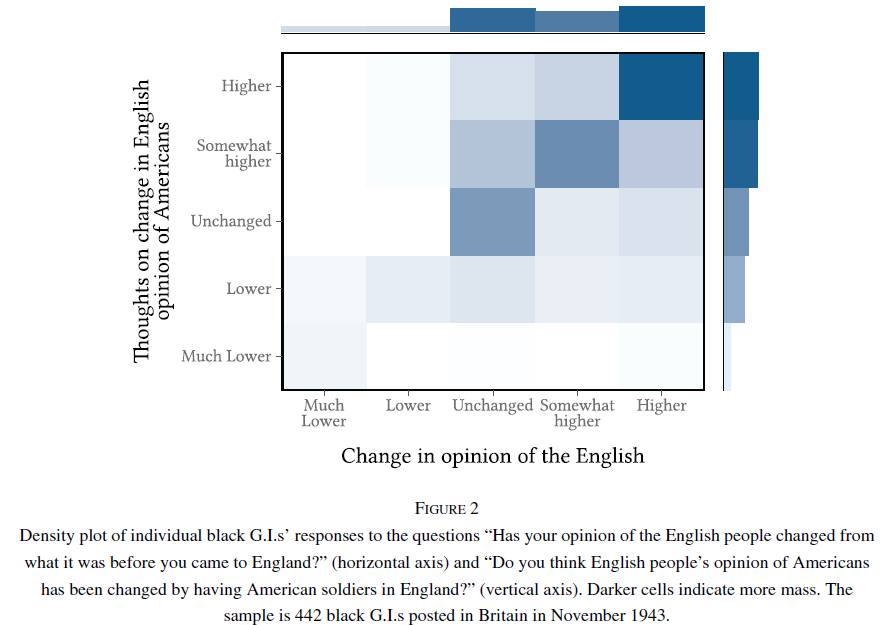
\includegraphics[scale = .4]{os1027tanji/F2}
    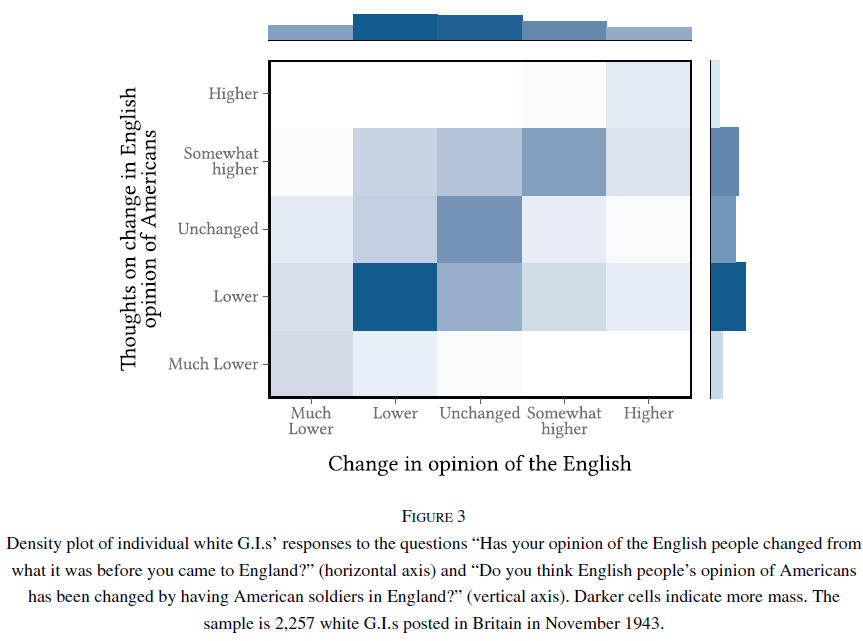
\includegraphics[scale = .4]{os1027tanji/F3}
  \end{figure}
\end{frame}

\begin{frame}\frametitle{Mass Observation}
  \begin{itemize}
    \item Qualitative evidence on British attitudes to the black troops.
    \item A UK-based survey organization founded in 1937 aiming to create an "anthropology of ourselves"
    \begin{itemize}
      \item A panel of volunteer respondents around the country
      \item Not designed to be representative of the population: consists largely of middle- and upper-class professionals.
    \end{itemize}
    \item In June 1943, the panel was asked about their personal attitude and effect of wartime events.
    \begin{itemize}
      \item 33 out of 199 (roughly 17\%) explicitly mentioned black troops.
      \item Eight responses (24\%) mention or imply contact with African American soldiers, of which six (75\%) show positive sentiment towards them.
      \item six responses explicitly report positive updating of attitudes or beliefs based on the presence of black troops, with only two implying negative updating.
    \end{itemize}
  \end{itemize}
\end{frame}

\section{Estimation Framework}
\frame{\sectionpage}
\begin{frame}\frametitle{Datasets}
  What to idenify: Persistent effects of presence of the black G.I.s on changes in local racial attitudes
  \begin{itemize}
    \item Local racial attitudes: three individual datasets with high geographical resolution
    \begin{enumerate}
      \item Membership of the BNP: a far-right xenophobic party
      \begin{itemize}
        \item across all of England andWales’ 180,000 census output areas
        \item collected by a national statistics agency
      \end{itemize}
      \item Voting outcomes from local elections
      \begin{itemize}
        \item 1973–2012
      \end{itemize}
      \item data generated by "Project Implicit"
      \begin{itemize}
        \item A website on which individuals can carry out a test for their implicit racial attitudes.
        \item individuals are prompted to provide self-reported racial attitudes and demographic information including their postcode.
      \end{itemize}
    \end{enumerate}
  \end{itemize}
\end{frame}

\begin{frame}\frametitle{}
  \begin{itemize}
    \item Troop Data
    \begin{itemize}
      \item A new data set of US army units in the UK (National Archives)
      \begin{itemize}
        \item based on the station lists produced by the US Army Adjutant Generals Office (AGO) on a monthly basis throughout the war, housed at the US National Archives in Washington D.C.
      \end{itemize}
      \item 27 digitized station lists (16 provided and 11 by themselves)
      \item Data period: June 1943 to December '45
      \item Units are listed along with the coordinates of the base at which:
      \begin{itemize}
        \item the unit was posted
        \item the nearest town or village
        \item a symbol to indicate if the unit is a segregated unit with African American troops
      \end{itemize}
      \item Typical units consists of around 150 men (called "company")
    \end{itemize}
    \item 1,937 military bases/camps (unique according to their coordinates) at 27 points in time: bases were located widely across England and Wales, with the notable exception of the South East of England.
  \end{itemize}
\end{frame}

\begin{frame}\frametitle{Identification}
  \begin{itemize}
    \item Assumption: the probability of locals' contact with troops increased in both the \# of troops and the length of station.
    \item Exogeneous valuation
    \begin{itemize}
      \item the time black troops were posted for and their numbers across space.
      \item the racial composition of support units across bases through time and space.
    \end{itemize}
    \item For each base $b$, the number of black units $\times$ months posted is expressed as:
    \[
    \textit{BlackUnitMonths}_b = \sum_m \textit{BlackSupportUnits}_{b, m}
    \]
    Similary, the measure for the presence of support troops:
    \[
    \textit{SupportUnitMonths}_b = \sum_m \textit{SupportUnits}_{b, m}
    \]
    $m$: months
  \end{itemize}
\end{frame}

\begin{frame}\frametitle{Checking Exogeneity}
  \begin{itemize}
    \item $\textit{BlackUnitMonths}_b$ is assumed to be exogeneous to pre-existing racial attitudes in the population, controlling $\textit{SupportUnitMonths}_b$.
    \begin{itemize}
      \item Non-differentiation policy of US Army European Theater of Operations.
      \item It would seem highly unlikely for race to have played a role in allocation decisions.
    \end{itemize}
    \item Regression of pre-existing economic, political, and geographic characteristics around that base.
    \[
    X_b = \alpha + \beta \textit{BlackUnitMonths}_b + \textit{SupportUnitMonths}_b + e_b
    \]
    \begin{itemize}
      \item Results are almost consistent with the idea that troop placements were made on the basis of military requirements, orthogonal to local conditions.
      \item Only the indicator for being inside an urban local government district was significant(at the 10\% level).
      \item Low F-statistic of F(25,524)=1.06 from a regression of $BlackUnitMonths$ on the full set of covariates.
    \end{itemize}
  \end{itemize}
\end{frame}

\begin{frame}\frametitle{}
  \begin{figure}
    \centering
    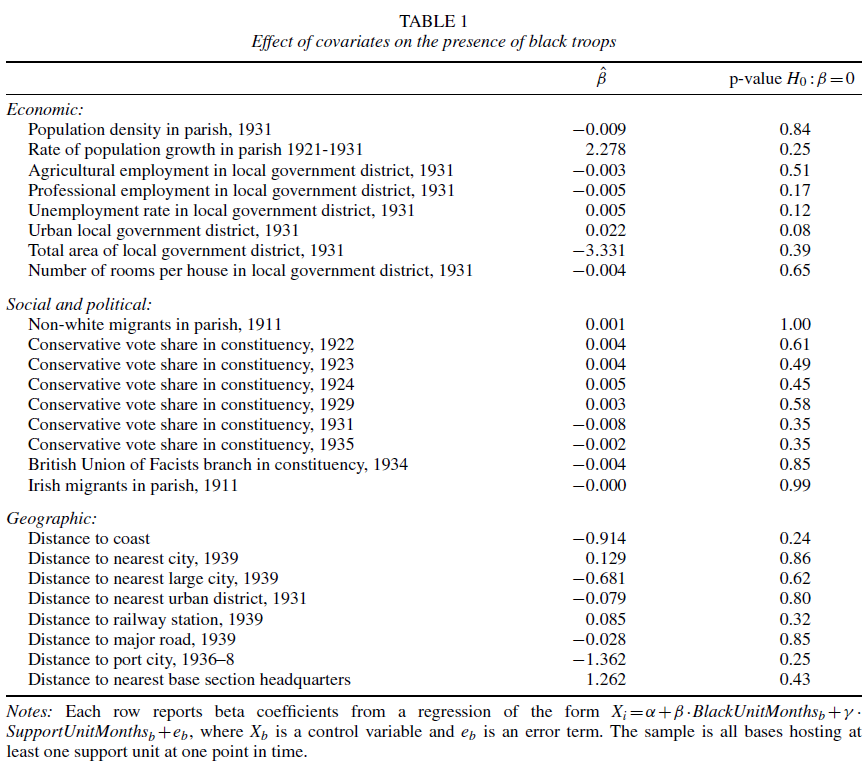
\includegraphics[scale = .6]{os1027tanji/T1}
  \end{figure}
\end{frame}

\begin{frame}\frametitle{Treatment Definition}
  \begin{itemize}
    \item A problem remained: how to match contemporary populations to historic bases.

    $\Rightarrow$ contemporary location to be "treated" by a given military base if the location and the military base share a common postcode district.
    \item For a postcode district $j$, the treatment is defined as:
    \begin{align*}
      \textit{BlackUnitMonths}_j &= \sum_b \sum_m \mathbb{1}[b \in j] \textit{BlackSupportUnits}_{b, m} \\
      \textit{SupportUnitMonths}_j &= \sum_j \sum_m \mathbb{1}[b \in j] \textit{SupportUnits}_{b, m}
    \end{align*}
    the intensity of presence of black and support troops around a given contemporary location.
  \end{itemize}
\end{frame}

\begin{frame}\frametitle{}
  \begin{figure}
    \centering
    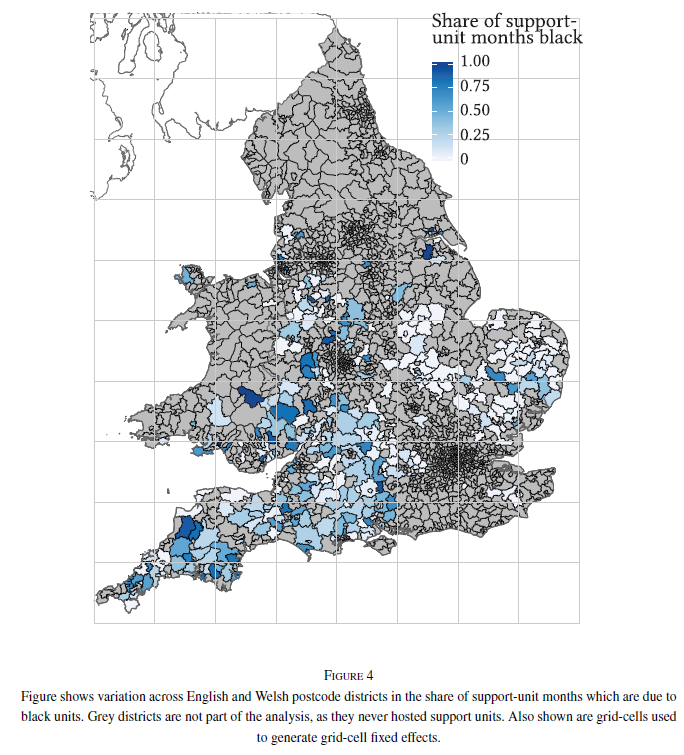
\includegraphics[scale = .6]{os1027tanji/F4}
  \end{figure}
\end{frame}

\section{Long-Term Effects on BNP Menbership}
\frame{\sectionpage}
\begin{frame}\frametitle{British National Party (BNP)}
  Local menbership of the BNP as a proxy for local attitudes.
  \begin{itemize}
    \item Far-right political party with extreme positions on race.
    \begin{itemize}
      \item founded in 1982 as a splinter group from the National Front.
      \item Police officers and prison officials were banned by their wmployers from joining the party.
    \end{itemize}
    \item A survey of YouGov (Goodwin and Evans, 2012) made a survey 2,951 supporters of the BNP, UK Independence Party, or the English Defence League.
    \begin{itemize}
      \item A large majority believes that immigrants are the main cause of crime and of disease.
      \item 47\% beloeve in innate differences in intelligence between black and white Britons.
    \end{itemize}
  \end{itemize}
\end{frame}

\begin{frame}\frametitle{Data construction}
  \begin{itemize}
    \item Biggs and Knauss (2011)'s data of geolocate members of the party using a membership list published online in 2008.
    \begin{itemize}
      \item confirmed by the party to be genuine and complete listing of menbers in November/December 2007.
      \begin{itemize}
        \item Membership of the BNP entailed some cost.
      \end{itemize}
      \item Information on 13,009 individuals, including a home address with a valid UK postcode in 97\% of cases.
      \item "Output area" level data from Biggs and Knauss (2011)
    \end{itemize}
    \item Data on the universe of the census output areas (neighbourhood) across England and Wales.
    \begin{itemize}
      \item 184,109 neighbourhoods (median population: 303)
      \item 12,513 (6.7\%) include at least one BNP member (max: 11).
      \item Membership of the BNP was geographically diverse.
    \end{itemize}
  \end{itemize}
\end{frame}

\begin{frame}\frametitle{Estimation and Results}
  \begin{itemize}
    \item Dependent variable: \# of BNP members per 100,000 white residents in a neighbourhood.
    \begin{align*}
      \textit{\# BNP} & \textit{members/100,000 whites}_i \\
      &= \alpha + \beta_1 \textit{BlackUnitMonths}_j
      + \beta_2 \textit{SupportUnitMonths}_j
      + \mathbf{X}_i + u_i \tag{1}
    \end{align*}
    \begin{itemize}
      \item $i$: neighbourhood, $j$: postcode district of the neighbourhood $j$
      \item $\mathbf{X}_i$: controls
      \item Standard errors at modern local authority level (348 administrative regions.)
      \item The parameter of interest: $\beta_1$
      \item Both the explanatory and dependent variables are standardized to have zero mean and a standard deviation of 1
    \end{itemize}
  \end{itemize}
\end{frame}

\begin{frame}\frametitle{Results}
  \begin{figure}
    \centering
    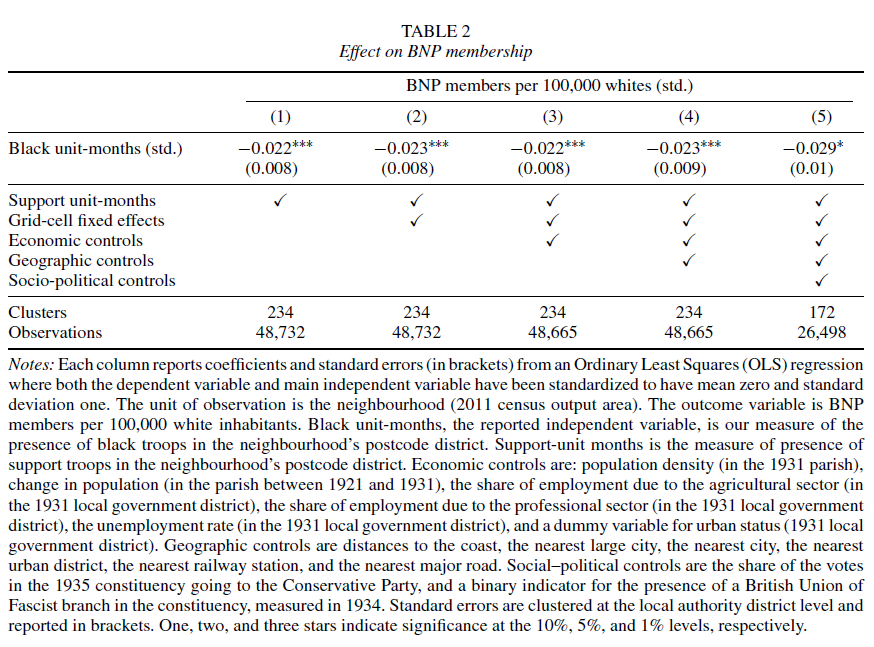
\includegraphics[scale = .6]{os1027tanji/T2}
  \end{figure}
\end{frame}

\begin{frame}\frametitle{}
  \begin{itemize}
    \item Concerns with the selection on unobservables.
    \item Oster (2019): the importance of movements in $R^2$.
    \begin{itemize}
      \item A relative degree of selection on observed and unobserved variables of $\delta = 34.51$, far above $\delta = 1$.
    \end{itemize}
  \end{itemize}
\end{frame}

\begin{frame}\frametitle{Robustness}
  \begin{figure}
    \centering
    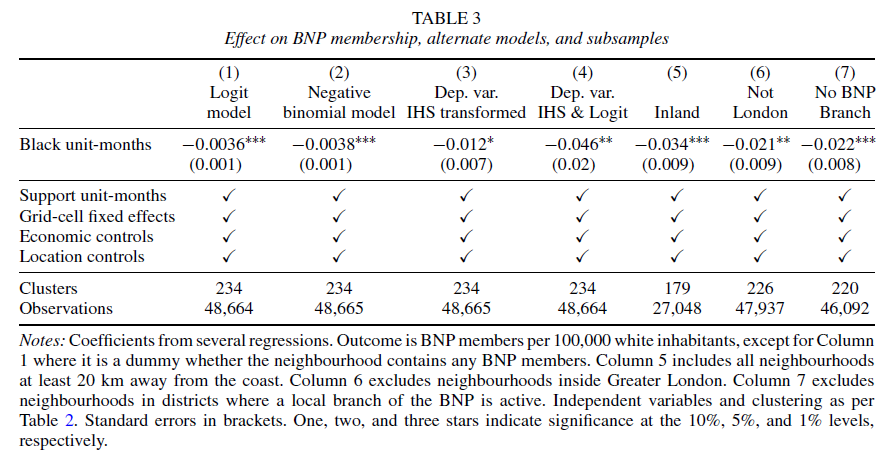
\includegraphics[scale = .6]{os1027tanji/T3}
  \end{figure}
\end{frame}

\begin{frame}\frametitle{Heterogeneity Analysis}
  \begin{figure}
    \centering
    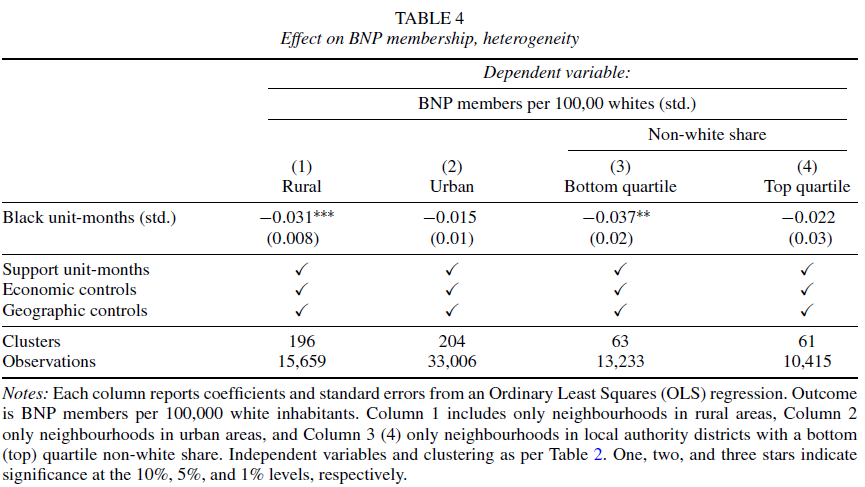
\includegraphics[scale = .6]{os1027tanji/T4}
  \end{figure}
  \begin{itemize}
    \scriptsize
    \item Rural areas of the UK see only low levels of internal migration.
    \item The effect of black G.I.s is almost twice as large in areas which are predominatly white.
    \item[cf.)] anti-Semitism in Germany across a period of 600 years "fails" in cities.
  \end{itemize}
\end{frame}

\begin{frame}\frametitle{Assessing the effect size}
  \begin{itemize}
    \item 1-standard deviation increase in black unit-months led to a .02 to .03 s.d. decrease in BNP membership:
    \begin{itemize}
      \item increasing all bases in a postcode district in a postcode district by in total 31 units $\times$ months decreases BNP membership by around 10\%.
    \end{itemize}
    \item The small effect sizes are the result of an intention-to-treat approach (ITT)
    \begin{itemize}
      \item Not every British person in the victiny of a US army base would have interacted with American troops.
      \item The effect might have worn off over time due to intergenerational decay.
    \end{itemize}
  \end{itemize}
\end{frame}

\begin{frame}\frametitle{}
  \begin{itemize}
    \item Average treatment effect on the treated (ATOT)
    \begin{enumerate}
      \item scale the ITT estimates by the share of the population directly exposed to the treatment.
      \begin{itemize}
        \item Survey by the US Army, "Attitudes Twards The British" (S - 122) asked how many English acquaintances the soldiers had.
        \item 23.54 British people per American soldier $\times$ 130,000 black G.I.s serving = 3.06 million (18.24\% out of the total population) had some interactions
        \item Considering overestimation: 9.12\% of the overall population had been treated

        $\Rightarrow$ .023 / 9.12\% = .252 standard deviation: ATOT.
      \end{itemize}
      \item incorporate the effets of decay among the treated population.
      \item analyse how spillover effects on the non-treated population could have influenced the ATOT estimate.
    \end{enumerate}
  \end{itemize}
\end{frame}

\begin{frame}\frametitle{}
  \begin{itemize}
    \item ATOT
    \begin{enumerate}
      \item scale the ITT estimates by the share of the population directly exposed to the treatment.

      \item incorporate the effets of decay among the treated population.
      \begin{itemize}
        \item Psychology: parent-child transmission rates of between .2 and .4 for racism in other countries (Duriez and Senens, 2009; Dhont and Van Hiel, 2012)
        \item Using .3 and four generations since WWII in 2010, the original effct was reduced to 23\%.
        $\Rightarrow$ 1.093 standard deviation
      \end{itemize}
      \item analyse how spillover effects on the non-treated population could have influenced the ATOT estimate.
    \end{enumerate}
  \end{itemize}
\end{frame}

\begin{frame}\frametitle{}
  \begin{itemize}
    \item ATOT
    \begin{enumerate}
      \item scale the ITT estimates by the share of the population directly exposed to the treatment.

      \item incorporate the effets of decay among the treated population.

      \item analyse how spillover effects on the non-treated population could have influenced the ATOT estimate.
      \begin{itemize}
        \item Spillover effects in various contexts to be typically of the order of 50\% of the original effect (Duflo and Saez, 2003; Nickerson, 2008; Angelucci and De Giorgi, 2009).
      \end{itemize}
      $\Rightarrow$ Using 25\%, the ATOTs are reduced to:
      \begin{itemize}
        \item .875 s.d. for the historical
        \item .202 s.d. for the contemporary population.
      \end{itemize}
    \end{enumerate}
  \end{itemize}
  More conservative estimate imply reasonably large effects both the time of treatment and in the present.
\end{frame}

\section{Additional Outcome Measures}
\frame{\sectionpage}
\begin{frame}\frametitle{Additional Outcome Measures}
  \begin{itemize}
    \item Three further measures of anti-minority prejudice to see the effect of black troops.
    \begin{itemize}
      \item It is also of interest whetther the presence of black G.I.s led to changes in attitudes more widely construed.
    \end{itemize}
    \begin{enumerate}
      \item Local election results
      \item Implicit attitudes
      \item Thermology
    \end{enumerate}
    \item Analyses are restricted to rural areas.
  \end{itemize}
\end{frame}

\begin{frame}\frametitle{Local Election Results}
  \begin{itemize}
    \item General election results only exist at the rather large Westminster constituency level
    \item Local government elections: \textit{The Elections Centre}
    \begin{itemize}
      \item taken between every 2 and for year.
      \item electoral ward level from 1973 to 2012.
    \end{itemize}
    \item Dependent variable: standardized vote share of BNP and Conservative parties in the rural areas.
    \item Voting results are discretized by time periods.
    \item[cf.)] It is not to say racial attitudes were ever the primary motivation for voting Conservative for the majority of their supporters.
  \end{itemize}
\end{frame}

\begin{frame}\frametitle{}
  \begin{figure}
    \centering
    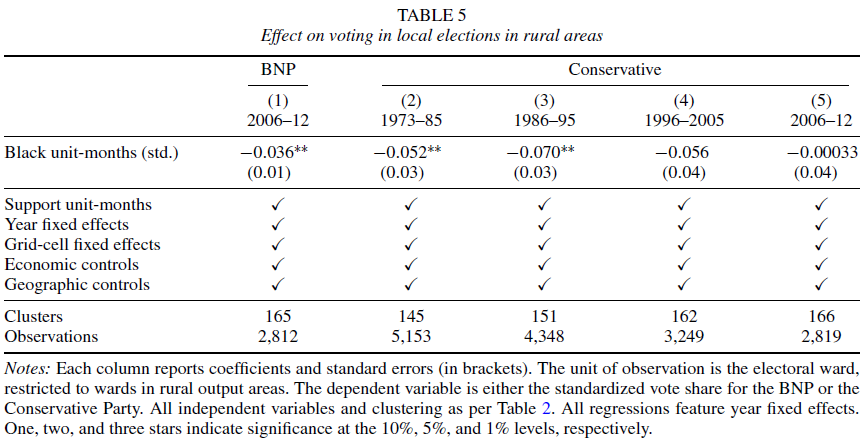
\includegraphics[scale = .6]{os1027tanji/T5}
  \end{figure}
  \begin{itemize}
    \footnotesize
    \item exposure to black troops depressed Conservative voting till about the early 2000s.
    \item With the widespread fielding of BNP candidates in the mid-2000s, this effect disappears.
    \begin{itemize}
      \scriptsize
      \item Large numbers of candidates from far-right parties only began to stand for election in the early 2000s.
      \item Racist ideologies were on view within parts of the Conservative Party during the mid-1960s.
    \end{itemize}
  \end{itemize}
\end{frame}

\begin{frame}\frametitle{Implicit Attitudes and Thermology}
  \begin{itemize}
    \item Implicit attitudes: measured by a computerized test have been shown to be redictive (Agerstr\"{o}m and Rooth, 2011)
    \item Data from Project Implicit (Xu et al., 2014): American NPO which hosts several country-specific websites allowing users to test their implicit attitudes using IAT.
    \begin{itemize}
      \item IAT: widely used in psychology (Greenwald et al., 1998)
      \item Individual "D" score on race (as well as gender, sexuality, weight,)
      \item About half of UK residents taking the IAT do so on Project  Implicit's US.
      \item 25,826 sessions with valid postcode data.
    \end{itemize}
    \item Thermology: survey questions after completing IAT.
    \begin{itemize}
      \item "Please rate how warm or cold you feel towards the following groups."; min = 0 (cold), max = 10 (warm)
    \end{itemize}
  \end{itemize}
\end{frame}

\begin{frame}\frametitle{}
  \begin{figure}
    \centering
    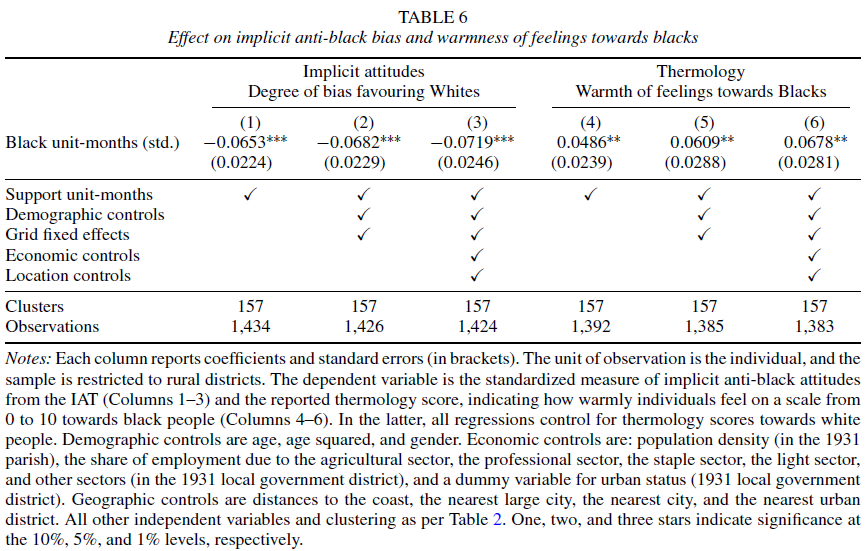
\includegraphics[scale = .6]{os1027tanji/T6}
  \end{figure}
\end{frame}


\section{Mechanism}
\frame{\sectionpage}
\begin{frame}\frametitle{Channels of Persistence}
  \begin{itemize}
    \item In order to better understand channels of persistence of the observed effect:
    \begin{itemize}
      \item Horizontal vs. Vertical  transmission
      \item Strengthening the contact hypothesis
    \end{itemize}
    \item Two steps of procedure:
    \begin{enumerate}
      \item Irish and non-white migration dampens the estimated treatment effect.
      \item Vertical transmission observed in some descriptive evidence by splitting the IAT results by birth cohorts.
    \end{enumerate}
  \end{itemize}
\end{frame}

\begin{frame}\frametitle{Irish and Non-White Migration}
  \begin{itemize}
    \item Neither existing Irish nor non-white migration to the UK by 1911 can predict where black units were stationed.
    \begin{itemize}
      \item Selection by the migrants where to choose, or contact between them and the population may have mitigated pre-existing racial prejudice.
      \item The further effects of contact can be reduced.
    \end{itemize}
    \item Splitting the sample into quartiles using the 1911 share of Irish migrants in a parish.
  \end{itemize}
\end{frame}

\begin{frame}\frametitle{}
  \begin{figure}
    \centering
    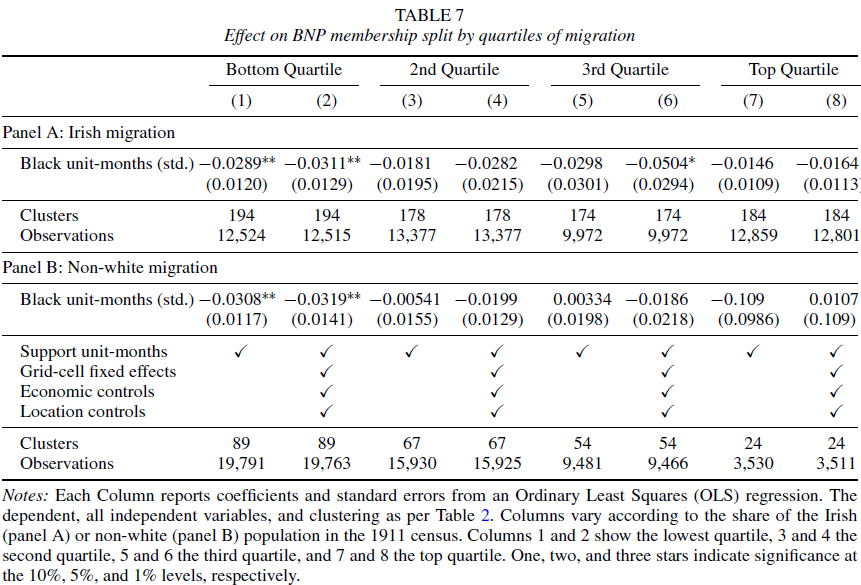
\includegraphics[scale = .6]{os1027tanji/T7}
  \end{figure}
\end{frame}

\begin{frame}\frametitle{IAT Splits}
  \begin{itemize}
    \item Urban/rural splits = vertical rather than transmission?
    \item IAT data contain information on teh age of participants: enable to divide them into birth cohorts.
    \begin{itemize}
      \item 1925-1940: directly affected cohorts
      \item 1960-1969: vertical transmission may occur

      The effect suggests generational jumps
    \end{itemize}
    \item Under horizontal transmission model, the effect is expected to be strong shortly after the initial treatment.
    \item Problem; small number of observations: lack of power.
  \end{itemize}
\end{frame}

\begin{frame}\frametitle{}
  \begin{figure}
    \centering
    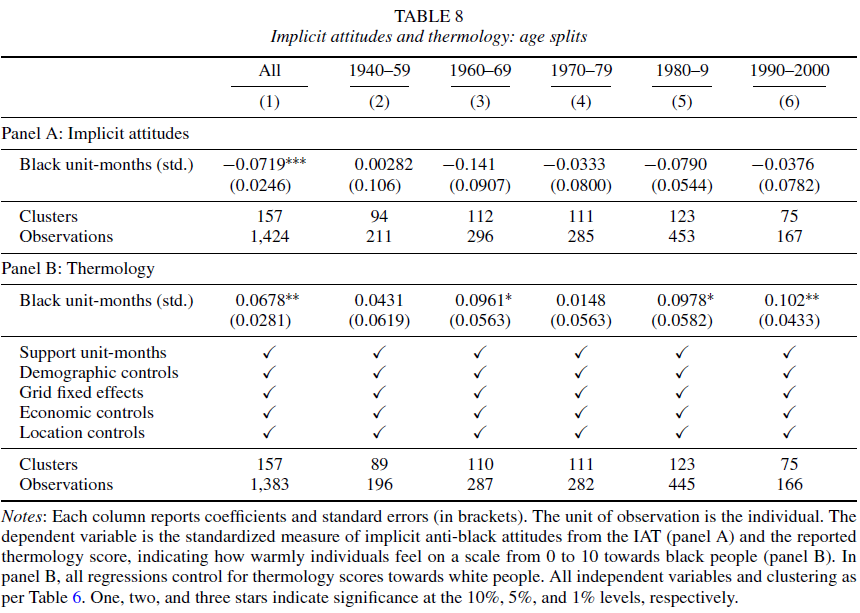
\includegraphics[scale = .6]{os1027tanji/T8}
  \end{figure}
\end{frame}

\section{Conclusion}
\frame{\sectionpage}
\begin{frame}\frametitle{Conclusion}
  \begin{itemize}
    \item This paper investigated the effect of the presence of black G.I.s diring WWII on anti-minority prrejudice.
    \begin{itemize}
      \item Exogeneous variation in allocation allows them to identify causal effects of the local presence of troops.
      \item Results support for the "contact hypothesis"(Allport, 1954).
    \end{itemize}
    \item What is interesting:
    \begin{itemize}
      \item The contact between the locals and the black G.I.s meets many of the conditions that Allport postulated were necessary for intergroup contact to lead to improved relations.
      \item Differences between updating towards white soldiers.
    \end{itemize}
  \end{itemize}
\end{frame}

\end{document}
